\documentclass[conference]{IEEEtran}
\IEEEoverridecommandlockouts

\usepackage{cite}
\usepackage{amsmath,amssymb,amsfonts}
\usepackage{algorithmic}
\usepackage{graphicx}
\usepackage{textcomp}
\usepackage{xcolor}
\usepackage[utf8]{vietnam}
\usepackage{booktabs}
\usepackage{multirow}
\usepackage{url}
\usepackage{tabularx}
\usepackage{tikz}
\usetikzlibrary{arrows.meta,positioning,shapes.geometric}

\renewcommand{\abstractname}{Tóm tắt nội dung}
\renewcommand{\IEEEkeywordsname}{Từ khóa}
\makeatletter
\renewenvironment{abstract}
{\normalfont\@IEEEabskeysecsize\bfseries\textit{\abstractname.}\quad\relax}
{\par\vspace{1.34ex}}
\renewenvironment{IEEEkeywords}
{\normalfont\@IEEEabskeysecsize\bfseries\textit{\IEEEkeywordsname.}\quad\relax}
{\par\vspace{0.67ex}}
\makeatother

\begin{document}

\title{Thiết kế môi trường học tăng cường SAC cho robot UR5e điều hướng quỹ đạo Cartesian trong tác vụ gắp-thả mô phỏng PyBullet}

\author{
\IEEEauthorblockN{1\textsuperscript{st} Liên Gia Bảo}
\IEEEauthorblockA{\textit{Khoa Kỹ thuật Điện tử 2}\\
\textit{Học viện Công nghệ Bưu chính Viễn thông}\\
TP. Hồ Chí Minh, Việt Nam\\
lienbao2k4@gmail.com}
\and
\IEEEauthorblockN{2\textsuperscript{nd} Lê Nguyễn Thái Bảo}
\IEEEauthorblockA{\textit{Khoa Kỹ thuật Điện tử 2}\\
\textit{Học viện Công nghệ Bưu chính Viễn thông}\\
TP. Hồ Chí Minh, Việt Nam\\
n22dcdk008@student.ptithcm.edu.vn}
}

\maketitle

\begin{abstract}
Bài báo trình bày chi tiết về thiết kế môi trường học tăng cường cho robot UR5e thực hiện tác vụ điều hướng quỹ đạo Cartesian phục vụ gắp và thả vật thể trong mô phỏng vật lý PyBullet. Tác vụ được mô hình hóa xấp xỉ theo quy trình quyết định Markov với không gian quan sát 20 chiều và không gian hành động liên tục 7 chiều (bao gồm 6 chiều điều khiển Cartesian thực tế và 1 chiều tay gắp dư thừa không được sử dụng trực tiếp do cơ chế tay gắp lai tự động). Thuật toán Soft Actor Critic được lựa chọn để huấn luyện chính sách điều hướng cho robot từ đầu mà không cần qua giai đoạn tiền huấn luyện. Nhằm giải quyết các thách thức về sự thưa thớt của phần thưởng và hiện tượng tối ưu hóa sai lệch, chúng tôi đề xuất cơ chế tay gắp lai tự động kích hoạt dựa trên khoảng cách vật lý, bộ ràng buộc tư thế đầu hút và hàm phần thưởng phân chia theo pha cụ thể. Hệ thống được cấu hình huấn luyện với ngân sách tối đa 10 triệu bước thời gian; các log đánh giá thực tế được sử dụng trong bài hiện có đến mốc 6.6 triệu bước, với cấu trúc vector hóa song song 16 môi trường và áp dụng chuẩn hóa VecNormalize. Kết quả đánh giá cho thấy từ mốc 600,000 bước, mô hình không ghi nhận episode thất bại trong 20 episode tại mỗi lần đánh giá, với điểm phần thưởng gốc trung bình đạt 570.20 và số bước thực thi trung bình là 28.65 bước. Kết quả này được ghi nhận trên một seed huấn luyện duy nhất (seed 42) và chỉ trên phân phối vật thể cấu hình \texttt{difficulty=1}. Checkpoint cuối 10 triệu bước không được sử dụng để lập đồ thị do không có log đánh giá tương ứng. Các kết quả cho thấy tính khả thi của phương pháp thiết kế môi trường và hàm thưởng trong việc hỗ trợ tác tử học quỹ đạo điều hướng trong cấu hình mô phỏng đang xét, đồng thời bài báo thảo luận thẳng thắn về các giới hạn hiện tại liên quan đến tính tổng quát của kết quả, chiều hành động dư thừa và khoảng cách giữa mô phỏng và thực tế.
\end{abstract}

\begin{IEEEkeywords}
Học tăng cường, Soft Actor Critic, UR5e, Pick and Place, PyBullet, Reward Shaping.
\end{IEEEkeywords}

\section{Giới thiệu}
Tác vụ gắp và thả vật thể là một trong những hoạt động cơ bản nhất của các hệ thống cánh tay robot công nghiệp. Trong môi trường sản xuất truyền thống, robot thường được lập trình để di chuyển qua các điểm tọa độ cố định được xác định trước. Tuy nhiên, phương pháp này gặp khó khăn khi vật thể xuất hiện ở các vị trí ngẫu nhiên hoặc có tư thế thay đổi liên tục. Khi đó, hệ thống điều khiển yêu cầu khả năng thích ứng cao để tự động tìm kiếm đường đi, tránh va chạm với các chướng ngại vật xung quanh, đồng thời đảm bảo tư thế tiếp cận của đầu công tác luôn chính xác để thực hiện gắp vật thể an toàn.

Học tăng cường sâu đã mở ra một hướng đi mới cho việc điều khiển robot bằng cách cho phép tác tử tự học chính sách điều khiển thông qua tương tác trực tiếp với môi trường mô phỏng vật lý \cite{kober2013reinforcement}. Thuật toán Soft Actor Critic (SAC) là một trong những thuật toán học tăng cường hiện đại nổi bật cho không gian hành động liên tục nhờ vào cơ chế tối đa hóa entropy phối hợp với mục tiêu tối ưu hóa phần thưởng tích lũy \cite{sutton2018reinforcement}. Cơ chế này giúp chính sách điều khiển giữ được tính khám phá cao, tránh rơi vào các cực trị địa phương trong quá trình huấn luyện và tối ưu hóa hiệu quả sử dụng mẫu thông qua replay buffer.

Mặc dù thuật toán học tăng cường có nền tảng lý thuyết vững chắc, việc triển khai thành công cho các tác vụ robot thực tế phụ thuộc rất lớn vào cách thức thiết kế môi trường. Các bài toán thao tác vật lý thường đối mặt với vấn đề phần thưởng rất thưa thớt nếu chỉ trao phần thưởng khi hoàn thành toàn bộ tác vụ. Ngược lại, nếu thiết kế phần thưởng quá dày đặc nhưng thiếu các ràng buộc vật lý, tác tử dễ tìm ra các hành vi lách luật để nhận điểm thưởng mà không thực sự hoàn thành mục tiêu gắp thả vật thể. Do đó, việc xây dựng một không gian trạng thái đầy đủ, không gian hành động hợp lý, kết hợp với các cơ chế điều khiển hướng đầu hút và phân chia pha phần thưởng là đóng góp trọng tâm của nghiên cứu này.

Trong bài báo này, chúng tôi tập trung vào việc mô hình hóa và thiết kế chi tiết môi trường học tăng cường cho robot UR5e 6 bậc tự do trong phần mềm mô phỏng PyBullet. Thay vì yêu cầu tác tử học đồng thời cả quỹ đạo di chuyển và thời điểm đóng mở tay gắp, chúng tôi đề xuất cơ chế tay gắp lai tự động hóa logic hút thả dựa trên điều kiện khoảng cách hình học, giúp tác tử tập trung vào việc tối ưu hóa quỹ đạo Cartesian. Đồng thời, bộ ràng buộc góc quay đầu hút được áp dụng để giữ cho giác hút luôn hướng xuống song song với mặt bàn. Hàm phần thưởng được thiết kế dựa trên ba pha hoạt động rõ rệt bao gồm: tiếp cận vật thể, nâng vật thể lên cao và di chuyển thả vật thể vào thùng chứa. Hệ thống được đánh giá chi tiết qua các đường cong học tập và thử nghiệm trong mô phỏng để ghi nhận tính ổn định trước khi thảo luận về các giới hạn và hướng phát triển trong tương lai.

\section{Nền tảng lý thuyết và Động học UR5e}

\subsection{Thuật toán Soft Actor Critic}
Soft Actor Critic \cite{haarnoja2018soft} là thuật toán học tăng cường dựa trên khung actor critic off policy, tối ưu hóa chính sách theo lý thuyết entropy tối đa. Mục tiêu huấn luyện không chỉ là tối đa hóa tổng phần thưởng mong đợi mà còn tối đa hóa entropy của chính sách để tăng cường khả năng khám phá không gian hành động:
\begin{equation}
J(\pi) = \sum_{t=0}^{T} \mathbb{E}_{(s_t,a_t)\sim\rho_\pi} \left[ r(s_t,a_t) + \alpha \mathcal{H}(\pi(\cdot|s_t)) \right]
\end{equation}
Trong đó $\mathcal{H}(\cdot)$ là hàm entropy của chính sách $\pi$, và $\alpha$ là tham số nhiệt độ quyết định mức độ ưu tiên của entropy so với phần thưởng thu được. Trong không gian hành động liên tục, chính sách được mô hình hóa bằng một phân phối Gaussian nhiều chiều với trung bình và độ lệch chuẩn được xuất ra từ mạng neural của actor.

Thuật toán SAC sử dụng hai mạng critic độc lập để ước lượng giá trị trạng thái hành động $Q_{\theta_1}(s, a)$ and $Q_{\theta_2}(s, a)$ nhằm giảm thiểu sự ước lượng quá cao của giá trị $Q$. Quá trình cập nhật các tham số mạng critic được thực hiện bằng cách tối thiểu hóa sai số Bellman:
\begin{equation}
L(\theta_i) = \mathbb{E}_{(s,a,r,s')\sim \mathcal{D}} \left[ \left( Q_{\theta_i}(s,a) - \left( r + \gamma V_{\bar{\psi}}(s') \right) \right)^2 \right]
\end{equation}
Hàm giá trị trạng thái mục tiêu $V_{\bar{\psi}}(s')$ được tính thông qua chính sách hiện tại và mạng critic mục tiêu được cập nhật chậm bằng phương pháp Polyak averaging với tham số $\tau$. Hệ số entropy $\alpha$ cũng được tự động điều chỉnh trong suốt quá trình học để duy trì một mức entropy tối thiểu mong muốn.

\subsection{Động học thuận robot UR5e}
Cánh tay robot UR5e gồm 6 khớp xoay kết nối liên tiếp từ đế robot đến đầu công tác \cite{ur5espec}. Để mô tả toán học mối quan hệ giữa góc khớp và vị trí trong không gian của đầu công tác, chúng tôi áp dụng quy tắc Denavit Hartenberg chuẩn (Standard DH Convention) \cite{hawkins2013analytic, andersen2018kinematics, craig2005introduction, spong2006robot}. Hệ tọa độ của từng khớp được thiết lập dọc theo các trục khớp xoay tương ứng.

\begin{figure*}[!t]
\centering
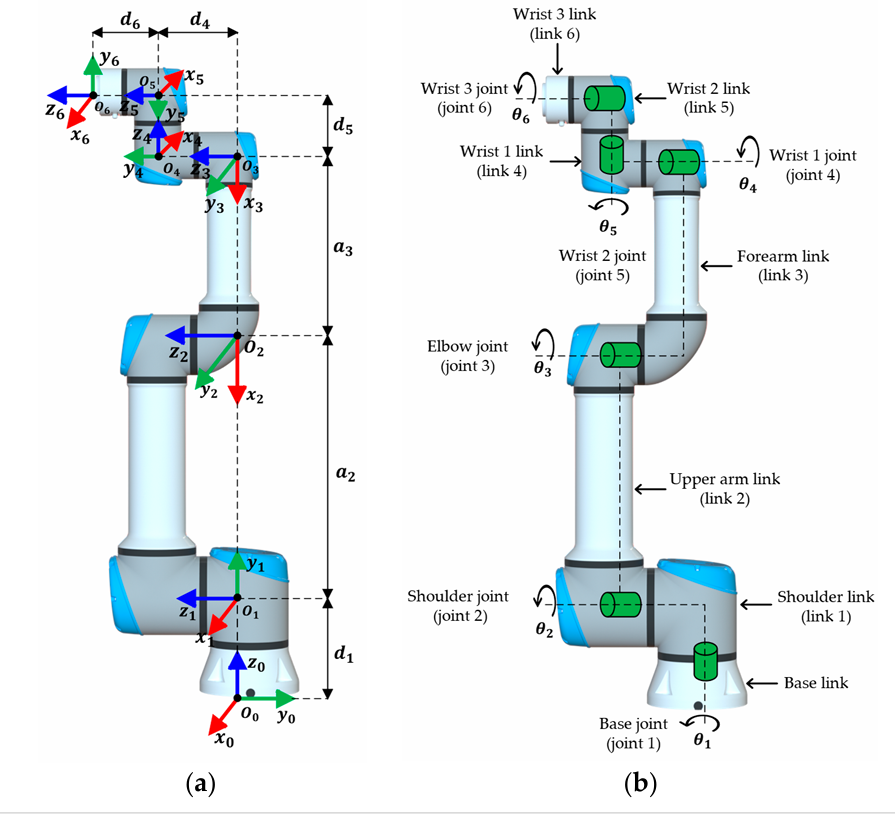
\includegraphics[width=0.70\textwidth]{figures/dh_frame_assignment.png}
\caption{Sơ đồ gán hệ trục DH và tên các khớp của robot UR5e dùng trong mô hình động học.}
\label{fig:dh_frame}
\end{figure*}

Hệ DH dùng trong phần động học là hệ tọa độ cục bộ của robot. Khi giao tiếp với PyBullet, hệ này được chuyển đổi sang hệ tọa độ world bằng phép xoay 180 độ quanh trục Z và cộng độ cao bàn 0.42 m. Bảng thông số DH của robot UR5e được trích xuất tự động từ tệp cấu hình \texttt{ur5e\_final.urdf} và được trình bày chi tiết trong Bảng~\ref{tab:dh}.

\begin{table*}[!t]
\caption{Bảng thông số Denavit Hartenberg của robot UR5e}
\label{tab:dh}
\centering
\begin{tabular}{@{}ccccc@{}}
\toprule
Khớp ($i$) & $a_i$ (m) & $d_i$ (m) & $\alpha_i$ (rad) & Offset khớp\\
\midrule
1 & 0.0000 & 0.1625 & $\pi/2$ & 0.0\\
2 & $-0.4250$ & 0.0000 & 0.0 & 0.0\\
3 & $-0.3922$ & 0.0000 & 0.0 & 0.0\\
4 & 0.0000 & 0.1333 & $\pi/2$ & 0.0\\
5 & 0.0000 & 0.0997 & $-\pi/2$ & 0.0\\
6 & 0.0000 & 0.0996 & 0.0 & 0.0\\
\bottomrule
\end{tabular}
\end{table*}
Các giá trị âm của $a_2$ và $a_3$ xuất phát từ chiều trục X theo quy ước DH, không biểu thị chiều dài vật lý âm.

Với mỗi khớp $i$, ma trận biến đổi thuần nhất $A_i^{i-1}$ biểu diễn hệ tọa độ của khớp $i$ trong hệ tọa độ của khớp $i-1$ được xác định theo công thức lượng giác tiêu chuẩn:
\begin{equation}
A_i^{i-1} = \begin{bmatrix}
\cos\theta_i & -\sin\theta_i\cos\alpha_i & \sin\theta_i\sin\alpha_i & a_i\cos\theta_i \\
\sin\theta_i & \cos\theta_i\cos\alpha_i & -\cos\theta_i\sin\alpha_i & a_i\sin\theta_i \\
0 & \sin\alpha_i & \cos\alpha_i & d_i \\
0 & 0 & 0 & 1
\end{bmatrix}
\end{equation}
Trong đó $\theta_i$ là góc xoay hiện tại của khớp $i$. Ma trận chuyển đổi tổng hợp từ đế robot đến đầu công tác $T_6^0$ được tính bằng tích tích lũy của 6 ma trận biến đổi thành phần:
\begin{equation}
T_6^0(q) = A_1^0(\theta_1) A_2^1(\theta_2) A_3^2(\theta_3) A_4^3(\theta_4) A_5^4(\theta_5) A_6^5(\theta_6)
\end{equation}
Cột cuối cùng của ma trận $T_6^0$ chứa tọa độ vị trí 3 chiều $(x_e, y_e, z_e)$ của đầu công tác trong hệ tọa độ cơ sở của robot, trong khi ma trận con $3 \times 3$ góc trên bên trái biểu diễn hướng xoay của đầu công tác dưới dạng ma trận quay $R_6^0$. Từ ma trận quay này, các góc Euler (Roll, Pitch, Yaw) được tính toán theo quy ước ZYX để phục vụ cho các thuật toán điều khiển và quan sát.

\subsection{Động học nghịch robot UR5e}
Bài toán động học nghịch yêu cầu xác định bộ góc khớp $q = [\theta_1, \theta_2, \theta_3, \theta_4, \theta_5, \theta_6]$ tương ứng với một vị trí và hướng đích của đầu công tác được mô tả bằng ma trận biến đổi đích $T_{target}$. Do robot UR5e có 3 khớp giữa ($\theta_2, \theta_3, \theta_4$) có các trục xoay song song với nhau, hệ thống điều khiển áp dụng phương pháp giải tích tách tâm cổ tay (Kinematic Decoupling) để giải bài toán một cách nhanh chóng và chính xác.

Đầu tiên, vị trí của tâm cổ tay (Wrist Center) được xác định bằng cách lùi một khoảng có chiều dài bằng $d_6$ dọc theo hướng trục $Z$ của đầu công tác:
\begin{equation}
P_{WC} = P_{target} - d_6 \cdot R_{target} \begin{bmatrix} 0 \\ 0 \\ 1 \end{bmatrix}
\end{equation}
Dựa trên hình học chiếu của $P_{WC}$ lên mặt phẳng XY, khớp vai thứ nhất $\theta_1$ được tính toán với hai cấu hình đối xứng đại diện cho hướng vai trái hoặc vai phải của robot:
\begin{equation}
\theta_1 = \text{atan2}(P_{WC,y}, P_{WC,x}) \pm \text{asin}\left(\frac{d_4}{\sqrt{P_{WC,x}^2 + P_{WC,y}^2}}\right)
\end{equation}
Tiếp theo, khớp cổ tay thứ hai $\theta_5$ được giải từ ma trận đích của hệ tọa độ đầu công tác:
\begin{equation}
\theta_5 = \pm \text{acos}\left(\frac{x_{target}\sin\theta_1 - y_{target}\cos\theta_1 - d_4}{d_6}\right)
\end{equation}
Sau khi xác định được $\theta_1$ và $\theta_5$, hướng của khớp cổ tay cuối cùng $\theta_6$ được tính bằng cách triệt tiêu ma trận xoay. Từ đó, ma trận biến đổi trung gian của các khớp giữa $T_{14}$ được xác định bằng cách nhân nghịch đảo:
\begin{equation}
T_{14} = (T_1)^{-1} T_{target} (A_5^4 A_6^5)^{-1}
\end{equation}
Nhờ vào tính chất song song của 3 khớp giữa, vị trí của khớp cổ tay thứ nhất trong mặt phẳng quay của cánh tay được giải bằng định lý hàm số Cosin cho tam giác tạo bởi bắp tay và cẳng tay:
\begin{equation}
\cos\theta_3 = \frac{x_{14}^2 + y_{14}^2 - a_2^2 - a_3^2}{2 a_2 a_3}
\end{equation}
Góc $\theta_3$ nhận hai giá trị tương ứng với cấu hình khuỷu tay hướng lên (Elbow Up) hoặc gập xuống (Elbow Down). Cuối cùng, hai góc $\theta_2$ và $\theta_4$ được tính toán từ các hệ phương trình lượng giác tuyến tính còn lại. Phương pháp giải tích này luôn tìm ra tối đa 8 nghiệm không gian khả thi chỉ trong khoảng thời gian dưới 1 mili-giây, giúp hệ thống hoạt động ổn định và tránh lỗi phân kỳ.

Trong trường hợp mục tiêu di chuyển nằm ở khu vực kỳ dị hoặc cận biên của vùng làm việc nơi phương pháp giải tích không tìm ra nghiệm thực, hệ thống tự động chuyển sang phương án dự phòng số học. Thuật toán tối ưu hóa \texttt{L-BFGS-B} được sử dụng để tối thiểu hóa hàm chi phí biểu diễn sai số vị trí và hướng:
\begin{equation}
E(q) = \| P_{curr}(q) - P_{target} \|^2 + \left(3.0 - \text{Tr}(R_{curr}(q) R_{target}^T)\right)
\end{equation}
Hàm tối ưu số học này giúp tìm ra cấu hình khớp gần đúng nhất trong phạm vi giới hạn xoay vật lý của robot.

\subsection{Kiểm chứng thuật toán động học tự xây dựng}
Bộ mã nguồn động học giải tích trong thư mục \texttt{kinematics} đóng vai trò là module kiểm chứng toán học độc lập, không tham gia vào vòng lặp điều khiển RL chính. Trong quá trình huấn luyện và suy diễn, môi trường RL sử dụng bộ giải động học nghịch tích hợp sẵn của PyBullet (hàm \texttt{calculateInverseKinematics}) để chuyển đổi lệnh Cartesian sang góc khớp vì lý do ổn định và tốc độ xử lý. Module giải tích tự xây dựng được sử dụng để kiểm chứng rằng mô hình DH của chúng tôi khớp chính xác với mô hình URDF mà PyBullet sử dụng. Để đảm bảo tính chính xác này, chúng tôi đã xây dựng hai kịch bản kiểm chứng tự động:
\begin{itemize}
    \item \textit{Kiểm chứng động học thuận}: So sánh tọa độ tính toán từ chuỗi nhân ma trận DH của chúng tôi với kết quả xuất ra trực tiếp từ thư viện PyBullet thông qua hàm \texttt{getLinkState} tại ba tư thế chính bao gồm tư thế 0 độ (Zero Pose), tư thế nghỉ (Home Pose) và tư thế đối xứng (Symmetry Pose). Kết quả kiểm thử thực tế đạt trạng thái thành công (PASS) với sai số vị trí bằng 0.000000 m, dưới tiêu chuẩn kiểm chứng quy định là 5 mm.
    \item \textit{Kiểm chứng động học nghịch}: Thực hiện kiểm chứng vòng lặp kín (Round Trip Verification) bằng cách chọn một bộ góc khớp ngẫu nhiên, đưa qua thuật toán động học thuận để tính vị trí đích, sau đó đưa vị trí đích này vào bộ giải động học nghịch để tìm lại góc khớp và tái đối chiếu vị trí. Bài kiểm tra này đạt trạng thái thành công (PASS) cho cả tư thế Home và các tư thế ngẫu nhiên với sai số Euclidean dưới $10^{-6}$ m (tiêu chuẩn quy định là dưới 1 mm). Đồng thời, bộ giải ghi nhận từ chối các tọa độ nằm ngoài tầm với vật lý của robot (ví dụ điểm tọa độ 5 m).
\end{itemize}

\subsection{Cơ chế điều khiển khớp và Cartesian trong môi trường RL}
Trong môi trường học tăng cường của nghiên cứu này, chính sách điều khiển không trực tiếp xuất ra giá trị góc xoay của 6 khớp robot. Thay vào đó, tác tử hoạt động trên không gian hành động Cartesian vi phân. Tại mỗi bước thời gian của vòng lặp điều khiển, tác tử sẽ đưa ra các giá trị dịch chuyển nhỏ delta vị trí và delta góc hướng của đầu công tác. Môi trường mô phỏng sẽ cộng các giá trị delta này vào tọa độ hiện tại của robot, thực hiện kẹp giới hạn trong không gian làm việc an toàn, sau đó gọi hàm \texttt{calculateInverseKinematics} của PyBullet để chuyển đổi sang bộ góc khớp mục tiêu. Cần lưu ý rằng bộ giải IK sử dụng trong vòng lặp RL là bộ giải số học tích hợp sẵn của PyBullet, khác với bộ giải giải tích tự xây dựng được mô tả ở Mục II.D chỉ phục vụ mục đích kiểm chứng. Cuối cùng, lệnh điều khiển vị trí khớp \texttt{POSITION\_CONTROL} được gửi đến các mô tơ của robot để thực hiện chuyển động vật lý có tính toán đến va chạm và lực cản. Cách tiếp cận này giúp đơn giản hóa đáng kể quá trình học tập của chính sách nhờ việc tận dụng cấu trúc hình học của không gian Cartesian.

\section{Thiết lập mô phỏng và Quy trình quyết định Markov}

\subsection{Cấu hình môi trường PyBullet}
Môi trường mô phỏng được xây dựng trong môi trường PyBullet \cite{coumans2021pybullet} bao gồm một robot UR5e đặt cố định trên một bàn làm việc, một vật thể hình trụ cần gắp và một thùng chứa mục tiêu để thả vật thể vào.
\begin{itemize}
    \item \textit{Bàn làm việc}: Có chiều cao chân bàn là 0.40 m, độ dày mặt bàn là 0.02 m. Mặt phẳng làm việc chính (TABLE\_SURFACE) có cao độ cố định là 0.42 m so với mặt đất. Đế robot được đặt tại vị trí $[0.0, 0.0, 0.42]$ m.
    \item \textit{Vùng an toàn cho đầu công tác (EE Workspace)}: Được giới hạn nghiêm ngặt để tránh va đập mạnh hoặc vượt quá tầm với vật lý của robot, cụ thể không gian hoạt động có giới hạn trục X từ 0.20 m đến 0.75 m, trục Y từ $-0.30$ m đến 0.30 m, và trục Z từ 0.44 m đến 0.95 m.
    \item \textit{Vật thể cần thao tác}: Là một khối hình trụ làm từ vật liệu mút xốp có bán kính đáy là 0.02 m, chiều cao thân trụ là 0.06 m và khối lượng tịnh là 0.1 kg. Hệ số ma sát trượt của vật thể được thiết lập ở mức 0.8 để đảm bảo sự ổn định khi kẹp gắp.
    \item \textit{Thùng chứa mục tiêu}: Được đặt cố định ở vị trí có tọa độ trọng tâm mặt bàn là $[0.65, -0.28, 0.42]$ m. Thùng chứa có thành cao 0.035 m bao quanh để ngăn vật thể bị trượt ra ngoài sau khi thả. Điểm đích để tính khoảng cách dẫn đường thả vật được thiết lập cao hơn đáy thùng 0.08 m (tức cao độ Z là 0.50 m) để dẫn hướng tay gắp đi từ phía trên miệng thùng xuống.
    \item \textit{Thông số vật lý mô phỏng}: Tần số mô phỏng của thế giới vật lý PyBullet được đặt ở mức chuẩn là 240 Hz (bước thời gian vật lý là 1/240 giây). Đối với vòng lặp học tăng cường, mỗi bước thực thi hành động của tác tử (RL Step) tương ứng với việc chạy liên tục 10 bước mô phỏng vật lý PyBullet (physics steps). Tần số điều khiển thực tế của tác tử do đó là 24 Hz, giúp đảm bảo các chuyển động diễn ra mượt mà và tránh các xung lực vật lý bất thường gây nổ mô phỏng.
\end{itemize}

\subsection{Quy luật sinh vật thể và các mức độ khó của môi trường}
Môi trường được thiết kế với ba cấu hình sinh vật thể có mức độ khó khác nhau nhằm phục vụ huấn luyện và đánh giá:
\begin{itemize}
    \item Mức \texttt{difficulty=0}: Vật thể chỉ được sinh ra trong một phạm vi hẹp có bán kính từ 0.12 m đến 0.25 m quanh vị trí nghỉ ban đầu của đầu gắp, đồng thời vật thể luôn được đặt thẳng đứng trên bàn.
    \item Mức \texttt{difficulty=1}: Phạm vi sinh vật thể được mở rộng từ 0.05 m đến 0.25 m. Đồng thời, có 50\% xác suất vật thể bị sinh ra ở tư thế nằm ngang ngẫu nhiên trên mặt bàn. Khi vật thể nằm ngang, tọa độ cao độ Z của vật thể được hạ thấp xuống mức TABLE\_SURFACE + 0.02 m (tương ứng với bán kính đáy) thay vì cao độ TABLE\_SURFACE + 0.033 m khi đặt đứng thẳng. Đây là cấu hình huấn luyện chính được sử dụng để thu thập các kết quả đánh giá trong báo cáo này.
    \item Mức \texttt{difficulty=2}: Vật thể được sinh ngẫu nhiên trong vùng làm việc của bàn (WORK\_ZONE) có giới hạn trục X từ 0.30 m đến 0.70 m, và giới hạn trục Y từ $-0.15$ m đến 0.15 m.
\end{itemize}

\subsection{Không gian quan sát}

\begin{table*}[!t]
\caption{Cấu trúc vector quan sát 20 chiều}
\label{tab:observation}
\centering
\scriptsize
\begin{tabularx}{\textwidth}{@{}ccX@{}}
\toprule
Chỉ số & Kích thước & Mô tả chi tiết thành phần quan sát\\
\midrule
$0 - 2$ & 3 & Tọa độ XYZ hiện tại của đầu công tác ($P_e$)\\
$3 - 5$ & 3 & Tọa độ XYZ hiện tại của vật thể hình trụ ($P_o$)\\
$6 - 8$ & 3 & Vector khoảng cách tương đối từ đầu công tác tới vật ($P_o - P_e$)\\
$9 - 11$ & 3 & Vector khoảng cách tương đối từ vật tới thùng chứa ($P_{bin} - P_o$)\\
$12 - 15$ & 4 & Quaternion biểu diễn góc xoay hướng của vật thể\\
16 & 1 & Trạng thái hoạt động của tay gắp (0.0: mở, 1.0: đóng)\\
$17 - 19$ & 3 & Các góc Euler (Roll, Pitch, Yaw) của đầu công tác\\
\bottomrule
\end{tabularx}
\end{table*}

Không gian quan sát của tác tử được thiết kế dưới dạng một vector liên tục 20 chiều, chứa các thông tin vị trí toàn cục, vị trí tương đối và thông số hướng của hệ thống robot vật thể. Chi tiết cấu trúc không gian quan sát được mô tả trong Bảng~\ref{tab:observation} \cite{gymnasiumspaces}. Cần lưu ý rằng vector quan sát này không bao gồm vận tốc khớp, vận tốc vật thể hay trạng thái pha hoạt động, do đó hệ thống gần đúng là một MDP xấp xỉ hơn là một MDP quan sát đầy đủ theo nghĩa chặt.

Việc đưa các vector tương đối vào không gian quan sát đóng vai trò quan trọng giúp mạng neural học được hàm giá trị nhanh chóng nhờ tín hiệu định hướng trực tiếp. Quaternion của vật thể giúp tác tử phân biệt rõ vật thể đang đứng hay nằm ngang để điều chỉnh góc tiếp cận, trong khi góc Euler của đầu công tác giúp tác tử nhận biết tư thế hiện tại để tự điều chỉnh về hướng thẳng đứng.

\subsection{Không gian hành động}
Hành động của tác tử là một vector liên tục 7 chiều, các giá trị thành phần được giới hạn trong miền $[-1.0, 1.0]$:
\begin{equation}
a_t = [\Delta x, \Delta y, \Delta z, \Delta \phi_r, \Delta \phi_p, \Delta \phi_y, a_{gripper}]
\end{equation}
Trong đó:
\begin{itemize}
    \item Ba thành phần đầu $[\Delta x, \Delta y, \Delta z]$ đại diện cho lệnh dịch chuyển tịnh tiến đầu công tác, được nhân với hệ số giới hạn hành trình CART\_DELTA\_MAX = 0.05 m để chuyển đổi sang kích thước mét thực tế.
    \item Ba thành phần tiếp theo $[\Delta \phi_r, \Delta \phi_p, \Delta \phi_y]$ đại diện cho lệnh thay đổi góc xoay cổ tay (Roll, Pitch, Yaw), được nhân với hệ số giới hạn góc xoay EULER\_DELTA\_MAX = 0.08 rad (tương đương khoảng 4.5 độ cho mỗi bước điều khiển).
    \item Thành phần thứ bảy $a_{gripper}$ được khai báo trong giao diện Gymnasium nhưng không tác động lên môi trường trong thiết kế hiện tại do logic gắp thả đã được tự động hóa bởi cơ chế tay gắp lai (Mục IV.A). Chiều hành động thứ bảy này được giữ lại trong vector hành động 7 chiều của mô hình hiện tại do giới hạn trong việc triển khai huấn luyện ban đầu và để thuận tiện cho các thử nghiệm mở rộng chế độ tự học tay gắp sau này. Chiều hành động thứ bảy không tạo ra tác động nhân quả lên trạng thái kế tiếp hoặc phần thưởng của môi trường. Do đó, về lý tưởng giá trị Q không phụ thuộc vào chiều này; tuy nhiên, việc duy trì nó vẫn làm tăng số chiều phân phối chính sách và có thể làm giảm hiệu quả khám phá. Như vậy, bậc tự do thực sự tác động lên hệ thống chỉ là 6 chiều Cartesian.
\end{itemize}


\begin{figure}[!t]
\centering
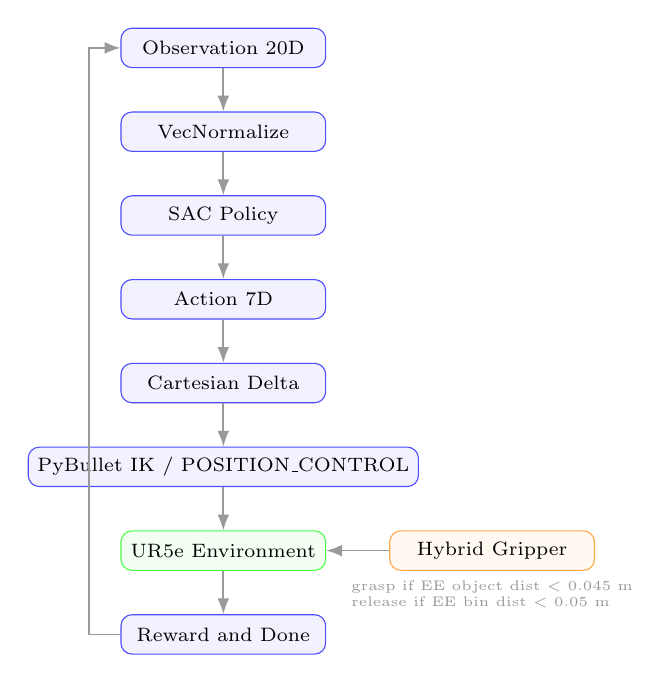
\begin{tikzpicture}[
    node distance=0.55cm,
    font=\scriptsize,
    box/.style={rectangle, draw=blue!70, fill=blue!5, rounded corners, align=center, minimum width=2.6cm, minimum height=0.5cm},
    env/.style={rectangle, draw=green!70, fill=green!5, rounded corners, align=center, minimum width=2.6cm, minimum height=0.5cm},
    gripper/.style={rectangle, draw=orange!70, fill=orange!5, rounded corners, align=center, minimum width=2.6cm, minimum height=0.5cm},
    arrow/.style={-Latex, draw=gray!80, semithick}
]
    % Node layout
    \node[box] (obs) {Observation 20D};
    \node[box, below=of obs] (norm) {VecNormalize};
    \node[box, below=of norm] (policy) {SAC Policy};
    \node[box, below=of policy] (act) {Action 7D};
    \node[box, below=of act] (delta) {Cartesian Delta};
    \node[box, below=of delta] (ik) {PyBullet IK / POSITION\_CONTROL};
    \node[env, below=of ik] (env) {UR5e Environment};
    \node[box, below=of env] (rew) {Reward and Done};
    
    % Gripper side-node
    \node[gripper, right=0.8cm of env] (grip) {Hybrid Gripper};
    
    % Connections
    \draw[arrow] (obs) -- (norm);
    \draw[arrow] (norm) -- (policy);
    \draw[arrow] (policy) -- (act);
    \draw[arrow] (act) -- (delta);
    \draw[arrow] (delta) -- (ik);
    \draw[arrow] (ik) -- (env);
    \draw[arrow] (env) -- (rew);
    
    % Feedback loop from reward/done to observation
    \draw[arrow] (rew.west) -- ++(-0.4,0) |- (obs.west);
    
    % Hybrid gripper connection to env
    \draw[arrow] (grip.west) -- (env.east);
    
    % Text notes under Hybrid Gripper
    \node[align=left, anchor=north, font=\tiny, text=gray!80] (notes) at (grip.south) {
        grasp if EE object dist < 0.045 m\\
        release if EE bin dist < 0.05 m
    };
\end{tikzpicture}
\caption{Sơ đồ pipeline điều khiển và học tăng cường của hệ thống.}
\label{fig:pipeline}
\end{figure}

\section{Thiết kế hệ thống Học tăng cường}

\subsection{Cơ chế tay gắp lai tự động}
Trong các tác vụ gắp thả sử dụng thuật toán học tăng cường, việc học đồng thời hai nhiệm vụ điều khiển vị trí liên tục và điều khiển logic đóng mở rời rạc của tay gắp thường dẫn đến hiệu suất huấn luyện kém. Tác tử có khả năng rơi vào tình trạng tối ưu hóa sai lệch (Reward Hacking) bằng cách đóng mở tay gắp liên tục ở gần vật thể để nhận điểm thưởng mà không di chuyển nâng vật. Để hạn chế vấn đề này, chúng tôi đề xuất cơ chế tay gắp lai (Hybrid Gripper) tự động hóa logic hoạt động của giác hút dựa trên phản hồi khoảng cách hình học từ mô phỏng. Cần nhận rõ rằng cơ chế này đơn giản hóa đáng kể bài toán: tác tử SAC chỉ cần học quỹ đạo di chuyển Cartesian của đầu công tác đến đúng vị trí, còn quyết định gắp và thả được tự động hóa bởi các quy tắc hình học cố định. Do đó, kết quả của nghiên cứu này phản ánh năng lực học điều hướng quỹ đạo trong môi trường có cơ chế gắp thả tự động, chứ không phải năng lực học toàn bộ chuỗi hành vi gắp thả tự chủ. Chi tiết cơ chế hoạt động như sau:
\begin{itemize}
    \item \textit{Pha kích hoạt}: Ở pha tiếp cận vật thể, giác hút chân không luôn được kích hoạt ở trạng thái chờ hút. Khi khoảng cách Euclidean giữa đầu công tác và vị trí vật thể giảm xuống dưới ngưỡng 0.045 m, môi trường mô phỏng sẽ tự động tạo ra một liên kết cứng (fixed constraint) trong PyBullet để dán chặt vật thể vào đầu công tác. Ngưỡng 0.045 m được tính toán để bù trừ phần sai lệch hình học khi vật thể nằm ngang và mô phỏng độ nén của giác hút cao su.
    \item \textit{Bù sai số vị trí}: Khi tạo liên kết, chúng tôi tính toán ma trận chuyển đổi tương đối giữa vị trí của vật và hệ trục tọa độ của đầu công tác để tránh hiện tượng ép cứng hai trọng tâm vật lý đè lên nhau, ngăn ngừa việc tích tụ lực va chạm đột ngột làm bắn văng vật thể khỏi bàn làm việc (Physics Explosion).
    \item \textit{Pha giải phóng}: Khi tác tử đã gắp được vật và di chuyển đầu công tác đến gần tâm thùng chứa mục tiêu trong phạm vi bán kính dưới 0.05 m, liên kết cứng sẽ tự động được xóa bỏ để vật rơi tự do dưới tác dụng của trọng lực mô phỏng.
\end{itemize}
Nhờ cơ chế này, mạng neural của tác tử không cần tối ưu thời điểm đóng mở tay gắp mà có thể tập trung vào việc học quỹ đạo pose Cartesian của đầu công tác.

\subsection{Ràng buộc hướng đầu công tác}
Giác hút chân không cần được giữ hướng vuông góc với mặt bàn để việc tiếp cận và hút vật thể đạt độ tin cậy cao nhất. Để đạt được điều này, chúng tôi áp dụng một bộ ràng buộc tư thế vật lý trực tiếp lên giá trị góc đích trước khi gửi đến bộ giải động học nghịch:
\begin{itemize}
    \item Góc Roll của đầu công tác trong hệ tọa độ thế giới được kẹp chặt quanh biên trị số $\pm\pi$ với dung sai dao động cho phép là $\pm15^\circ$ ($\pm\pi/12$ rad).
    \item Góc Pitch được kẹp quanh trị số 0 với dung sai cho phép là $\pm15^\circ$ ($\pm\pi/12$ rad).
    \item Góc Yaw được thả tự do trong khoảng từ $-\pi$ đến $\pi$ để robot có thể tự do xoay cổ tay tiếp cận vật.
\end{itemize}
Bộ ràng buộc này đóng vai trò như một bộ lọc hành động trực tiếp. Nó giúp hạn chế các tư thế xoắn ngược tay gắp không tự nhiên của robot, giảm không gian tìm kiếm nghiệm của bộ giải động học nghịch, đồng thời hỗ trợ ngăn ngừa hiện tượng tay gắp bị vặn xoắn nhiều vòng gây kẹt khớp vật lý.

\subsection{Thiết kế hàm phần thưởng phân chia theo pha}
Hàm phần thưởng được xây dựng dưới dạng các phần thưởng định hướng (Dense Reward) kết hợp phần thưởng sự kiện (Sparse Bonus), phân chia rõ rệt thành ba pha hoạt động dựa trên trạng thái của hệ thống:
\begin{itemize}
    \item \textit{Pha 0 (Tiếp cận vật)}: Khi robot chưa gắp được vật thể, phần thưởng khuyến khích đầu công tác tiến lại gần vật thể theo tỷ lệ khoảng cách:
    \begin{equation}
    r_{approach} = \max\left(0.0, 2.0 - 8.0 \cdot \| P_e - P_o \|\right)
    \end{equation}
    Khi khoảng cách đạt dưới ngưỡng gắp và liên kết được thiết lập thành công, tác tử nhận một điểm thưởng gắp vật lớn $+50.0$ điểm và hệ thống chuyển sang Pha 1.
    \item \textit{Pha 1 (Nâng và vận chuyển)}: Khi tác tử đã giữ được vật thể, hệ thống kiểm tra cao độ của vật thể. Nếu vật thể được nâng cao hơn mặt bàn ít nhất 0.20 m, tác tử được nhận một điểm thưởng nâng vật duy nhất là $+30.0$ điểm. Để ngăn ngừa tác tử kéo lê vật thể trên mặt bàn gây va chạm nguy hiểm, một hình phạt nghiêm khắc $-3.0$ điểm sẽ được áp dụng tại mỗi bước thời gian nếu vật thể đã được nâng nhưng cao độ đầu công tác bị hạ thấp dưới mức CARRY\_Z\_MIN = 0.60 m. Trong pha này, phần thưởng định hướng dẫn đường vật thể tiến về phía thùng chứa theo mặt phẳng ngang XY:
    \begin{equation}
    r_{carry} = \max\left(0.0, 2.0 - 5.0 \cdot \| P_{o,xy} - P_{bin,xy} \|\right)
    \end{equation}
    Khi vật thể tiến sát vào vùng không gian phía trên miệng thùng chứa trong bán kính dưới 0.15 m theo phương XY, hệ thống chuyển sang Pha 2.
    \item \textit{Pha 2 (Thả vật vào thùng)}: Khi đã đưa vật đến sát thùng chứa, phần thưởng khuyến khích tác tử hạ thấp đầu công tác để đưa vật thể vào sâu trong lòng thùng chứa:
    \begin{equation}
    r_{place} = \max\left(0.0, 3.0 - 10.0 \cdot \| P_e - P_{bin} \|\right)
    \end{equation}
    Khi điều kiện hoàn thành tác vụ được thỏa mãn, tức là vật thể nằm gọn trong thùng chứa với sai số khoảng cách so với tâm thùng đạt $\|P_{o,xy} - P_{bin,xy}\| < 0.05$ m và cao độ vật thể nằm dưới ngưỡng $z_o < 0.55$ m (tương ứng với TABLE\_SURFACE + 0.13 m), tác tử sẽ nhận điểm thưởng thành công cuối cùng rất lớn là $+500.0$ điểm và episode kết thúc.
    \item \textit{Phạt thời gian (Time Penalty)}: Tại mỗi bước thời gian của mô phỏng, một hình phạt cố định là $-0.05$ điểm được áp dụng nhằm thúc đẩy tác tử tìm kiếm quỹ đạo ngắn hơn và hoàn thành tác vụ trong ít bước hơn. Số bước tối đa cho một chu kỳ huấn luyện (MAX\_STEPS) là 300 bước.
\end{itemize}

\section{Thiết lập huấn luyện}
Chúng tôi thực hiện huấn luyện tác tử SAC từ đầu bằng cách sử dụng thư viện Stable Baselines3 \cite{raffin2021stable, sb3sac} trên nền tảng PyTorch. Để đảm bảo tốc độ thu thập dữ liệu huấn luyện và tính ổn định của gradient, hệ thống sử dụng cấu trúc vector hóa song song \texttt{SubprocVecEnv} với 16 tiến trình môi trường chạy đồng thời trên CPU. 

Toàn bộ các giá trị quan sát của môi trường và điểm số phần thưởng đều được đi qua bộ lọc \texttt{VecNormalize} \cite{sb3vec} để chuẩn hóa động về phân phối có trung bình bằng 0 và độ lệch chuẩn bằng 1 dựa trên các thống kê chạy tích lũy. Giá trị quan sát sau chuẩn hóa được kẹp chặt trong khoảng giới hạn $[-10.0, 10.0]$ để loại bỏ các điểm dị thường. Quá trình đánh giá chính sách được thực hiện tự động sau mỗi 200,000 bước huấn luyện tổng cộng (tương ứng với 12,500 bước trên mỗi môi trường song song) thông qua lớp \texttt{EvalCallback}. Mỗi lần đánh giá chạy 20 episode độc lập để tính toán tỷ lệ thành công trung bình. Bộ siêu tham số chi tiết được thiết lập tối ưu cho phần cứng và tác vụ được trình bày trong Bảng~\ref{tab:hyperparameters}.

\begin{table}[!t]
\caption{Siêu tham số huấn luyện chi tiết của thuật toán SAC}
\label{tab:hyperparameters}
\centering
\scriptsize
\begin{tabularx}{\columnwidth}{@{}p{0.44\columnwidth}X@{}}
\toprule
Siêu tham số & Giá trị tối ưu\\
\midrule
Mạng chính sách Actor & MLP $[256, 256]$\\
Mạng giá trị Critic & MLP $[256, 256]$\\
Hàm kích hoạt & ReLU\\
Tần số cập nhật & 1 bước cập nhật sau mỗi bước mô phỏng\\
Learning rate & $3 \cdot 10^{-4}$ (Hệ số Adam)\\
Hệ số chiết khấu $\gamma$ & 0.99\\
Kích thước lô mẫu & 256\\
Replay buffer & $1,000,000$ bước mẫu\\
Tham số cập nhật chậm $\tau$ & 0.005\\
Entropy coefficient & Tự động điều chỉnh (\texttt{auto\_0.1})\\
Mức độ khó huấn luyện & \texttt{difficulty=1}\\
Thiết bị & CPU/GPU tự động nhận diện\\
\bottomrule
\end{tabularx}
\end{table}

Cần chú ý rằng toàn bộ chính sách được cấu hình huấn luyện với ngân sách tối đa 10 triệu bước mẫu trên tệp \texttt{train\_17d\_place.py} với một seed ngẫu nhiên duy nhất (seed 42). Các log đánh giá thực tế được sử dụng trong bài hiện có đến mốc 6.6 triệu bước (checkpoint cuối 10 triệu bước không được sử dụng để lập đồ thị do không có log đánh giá tương ứng). Các điểm phần thưởng báo cáo trong phần kết quả là giá trị gốc trước khi qua bộ lọc VecNormalize. Chúng tôi không sử dụng các kỹ thuật huấn luyện chuyển tiếp hay nạp trước trọng số từ các giai đoạn huấn luyện gắp trước đó, cho thấy hàm phần thưởng thiết kế có thể hỗ trợ tác tử học quỹ đạo điều hướng trong cấu hình mô phỏng đang xét.

\section{Kết quả thực nghiệm và Thảo luận}

\subsection{Đánh giá tiến trình huấn luyện qua các đường cong học tập}
Tiến trình học tập của tác tử SAC được ghi nhận thông qua tệp dữ liệu đánh giá thực tế \texttt{evaluations.npz} được lưu trữ trong thư mục huấn luyện của seed 42. Đường cong học tập thu được bao gồm 3 đồ thị thành phần được trực quan hóa chi tiết trong Hình~\ref{fig:eval_curves}.

\begin{figure*}[!t]
\centering
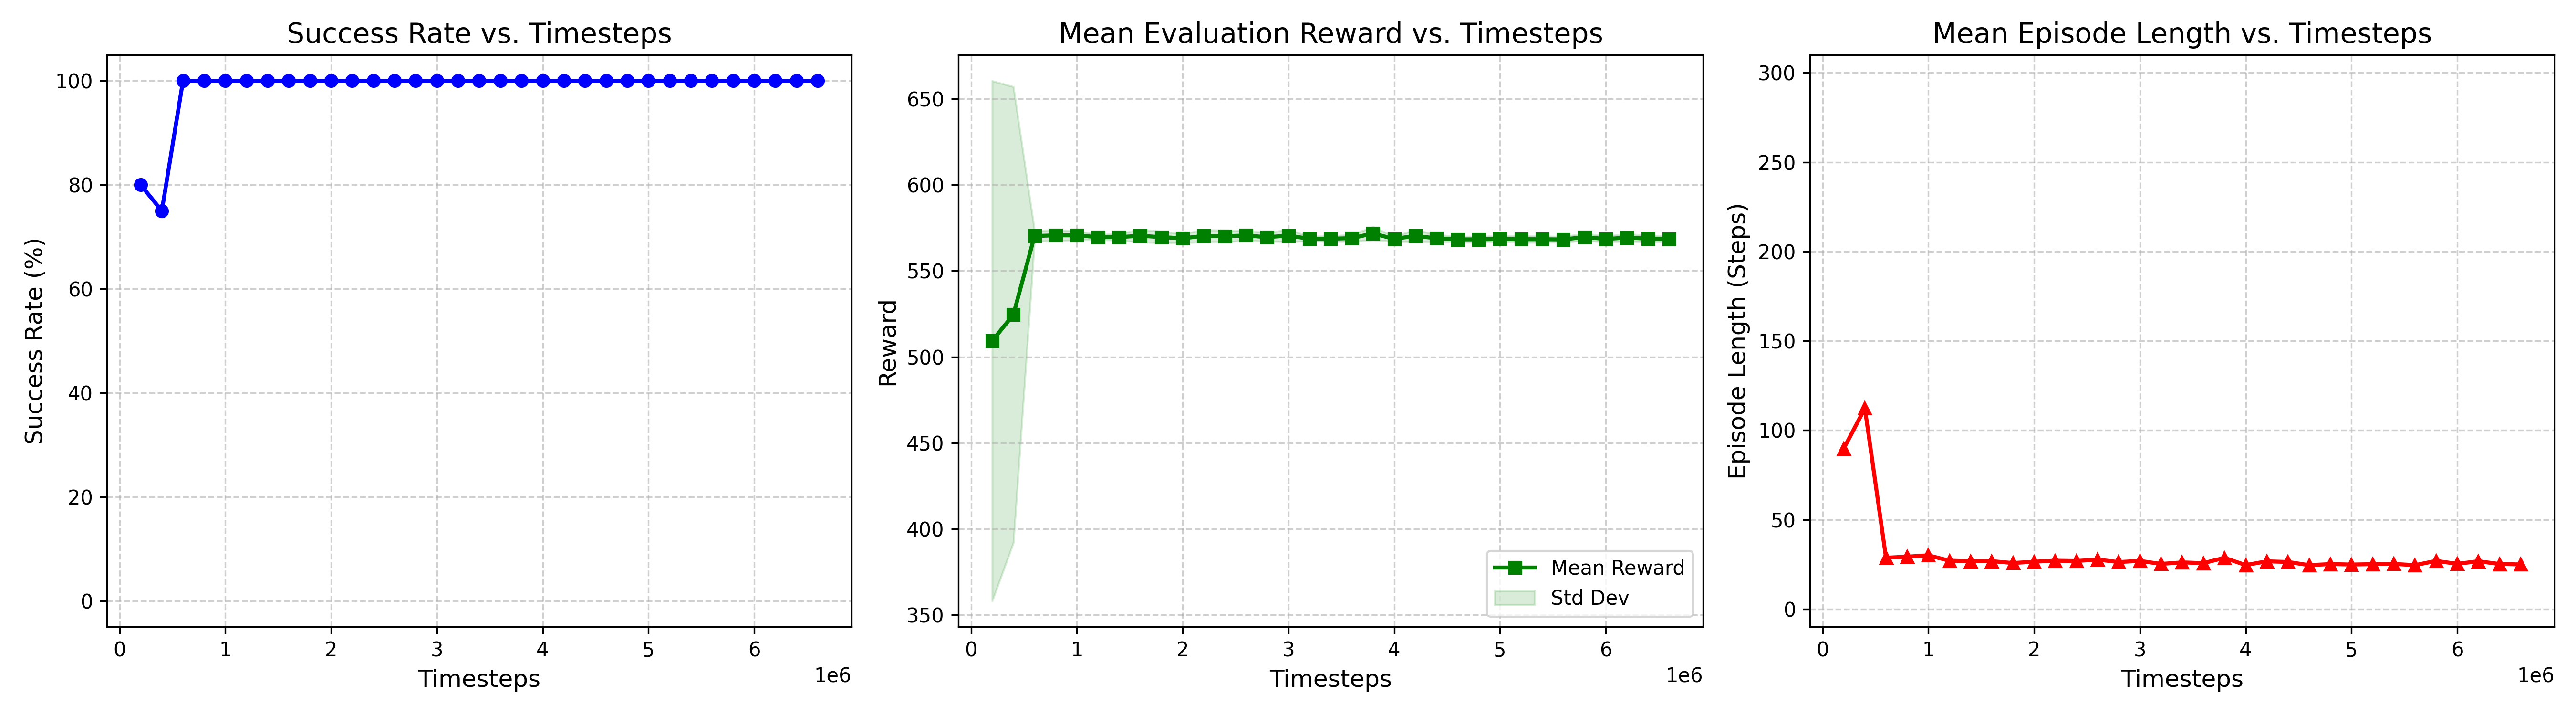
\includegraphics[width=0.98\textwidth]{figures/eval_curves.png}
\caption{Đường cong kết quả đánh giá tác tử SAC theo số bước huấn luyện bao gồm tỷ lệ thành công (trái), điểm phần thưởng trung bình với dải sai số lệch chuẩn (giữa) và chiều dài chu kỳ trung bình (phải).}
\label{fig:eval_curves}
\end{figure*}

Phân tích số liệu từ tệp đánh giá thực tế cho thấy các đặc điểm phát triển chính sách rất rõ ràng qua các giai đoạn học tập:
\begin{itemize}
    \item \textit{Giai đoạn khởi đầu (Dưới 400,000 bước)}: Tác tử đang tích cực khám phá không gian hoạt động. Tại mốc 200,000 bước thời gian, tỷ lệ thành công gắp thả đạt mức 80.0\% với điểm phần thưởng trung bình là 509.29 và số bước thực hiện trung bình khá cao là 89.70 bước. Tại mốc 400,000 bước, do tác tử tiếp tục khám phá các khu vực hành động mới nên hiệu suất có sự biến động nhẹ với tỷ lệ thành công đạt 75.0\%, điểm số phần thưởng trung bình là 524.46 và chiều dài chu kỳ tăng lên 112.25 bước.
    \item \textit{Giai đoạn hội tụ (Từ mốc 600,000 bước)}: Tại mốc đánh giá 600,000 bước thời gian, tác tử đã hội tụ về chính sách ổn định. Lần đánh giá định kỳ gồm 20 episode không ghi nhận episode thất bại (trong số 20 episode tại lần đánh giá đó) và kết quả này được duy trì ổn định. Điểm số phần thưởng trung bình đạt mức cao và ổn định là 570.20 với độ lệch chuẩn ở mức nhỏ là 3.08. Chiều dài chu kỳ thực hiện trung bình giảm mạnh xuống còn 28.65 bước, cho thấy tác tử đã di chuyển theo các đường đi thẳng ngắn hơn để thả vật.
    \item \textit{Giai đoạn ổn định lâu dài (Đến 6,600,000 bước)}: Khi tiếp tục huấn luyện kéo dài đến mốc 6,600,000 bước thời gian trong log đánh giá hiện có, chính sách tiếp tục không ghi nhận episode thất bại trong 20 episode tại mỗi lần đánh giá. Chiều dài chu kỳ trung bình dao động quanh mức 24.90 bước, với điểm phần thưởng ổn định ở mức 568.45 và độ lệch chuẩn ở mức 1.63. Điều này cho thấy thuật toán SAC kết hợp với chuẩn hóa VecNormalize có khả năng duy trì độ ổn định chính sách cao, không ghi nhận hiện tượng suy thoái chính sách khi huấn luyện lâu dài.
\end{itemize}

\subsection{Trực quan hóa chuỗi hoạt động thực thi của robot}
Chuỗi hành vi hoàn chỉnh của robot UR5e khi thực hiện gắp thả một vật thể nằm ngang trong mô phỏng vật lý PyBullet được trực quan hóa qua 4 pha chính trong Hình~\ref{fig:demo_sequence}.

\begin{figure*}[!t]
\centering
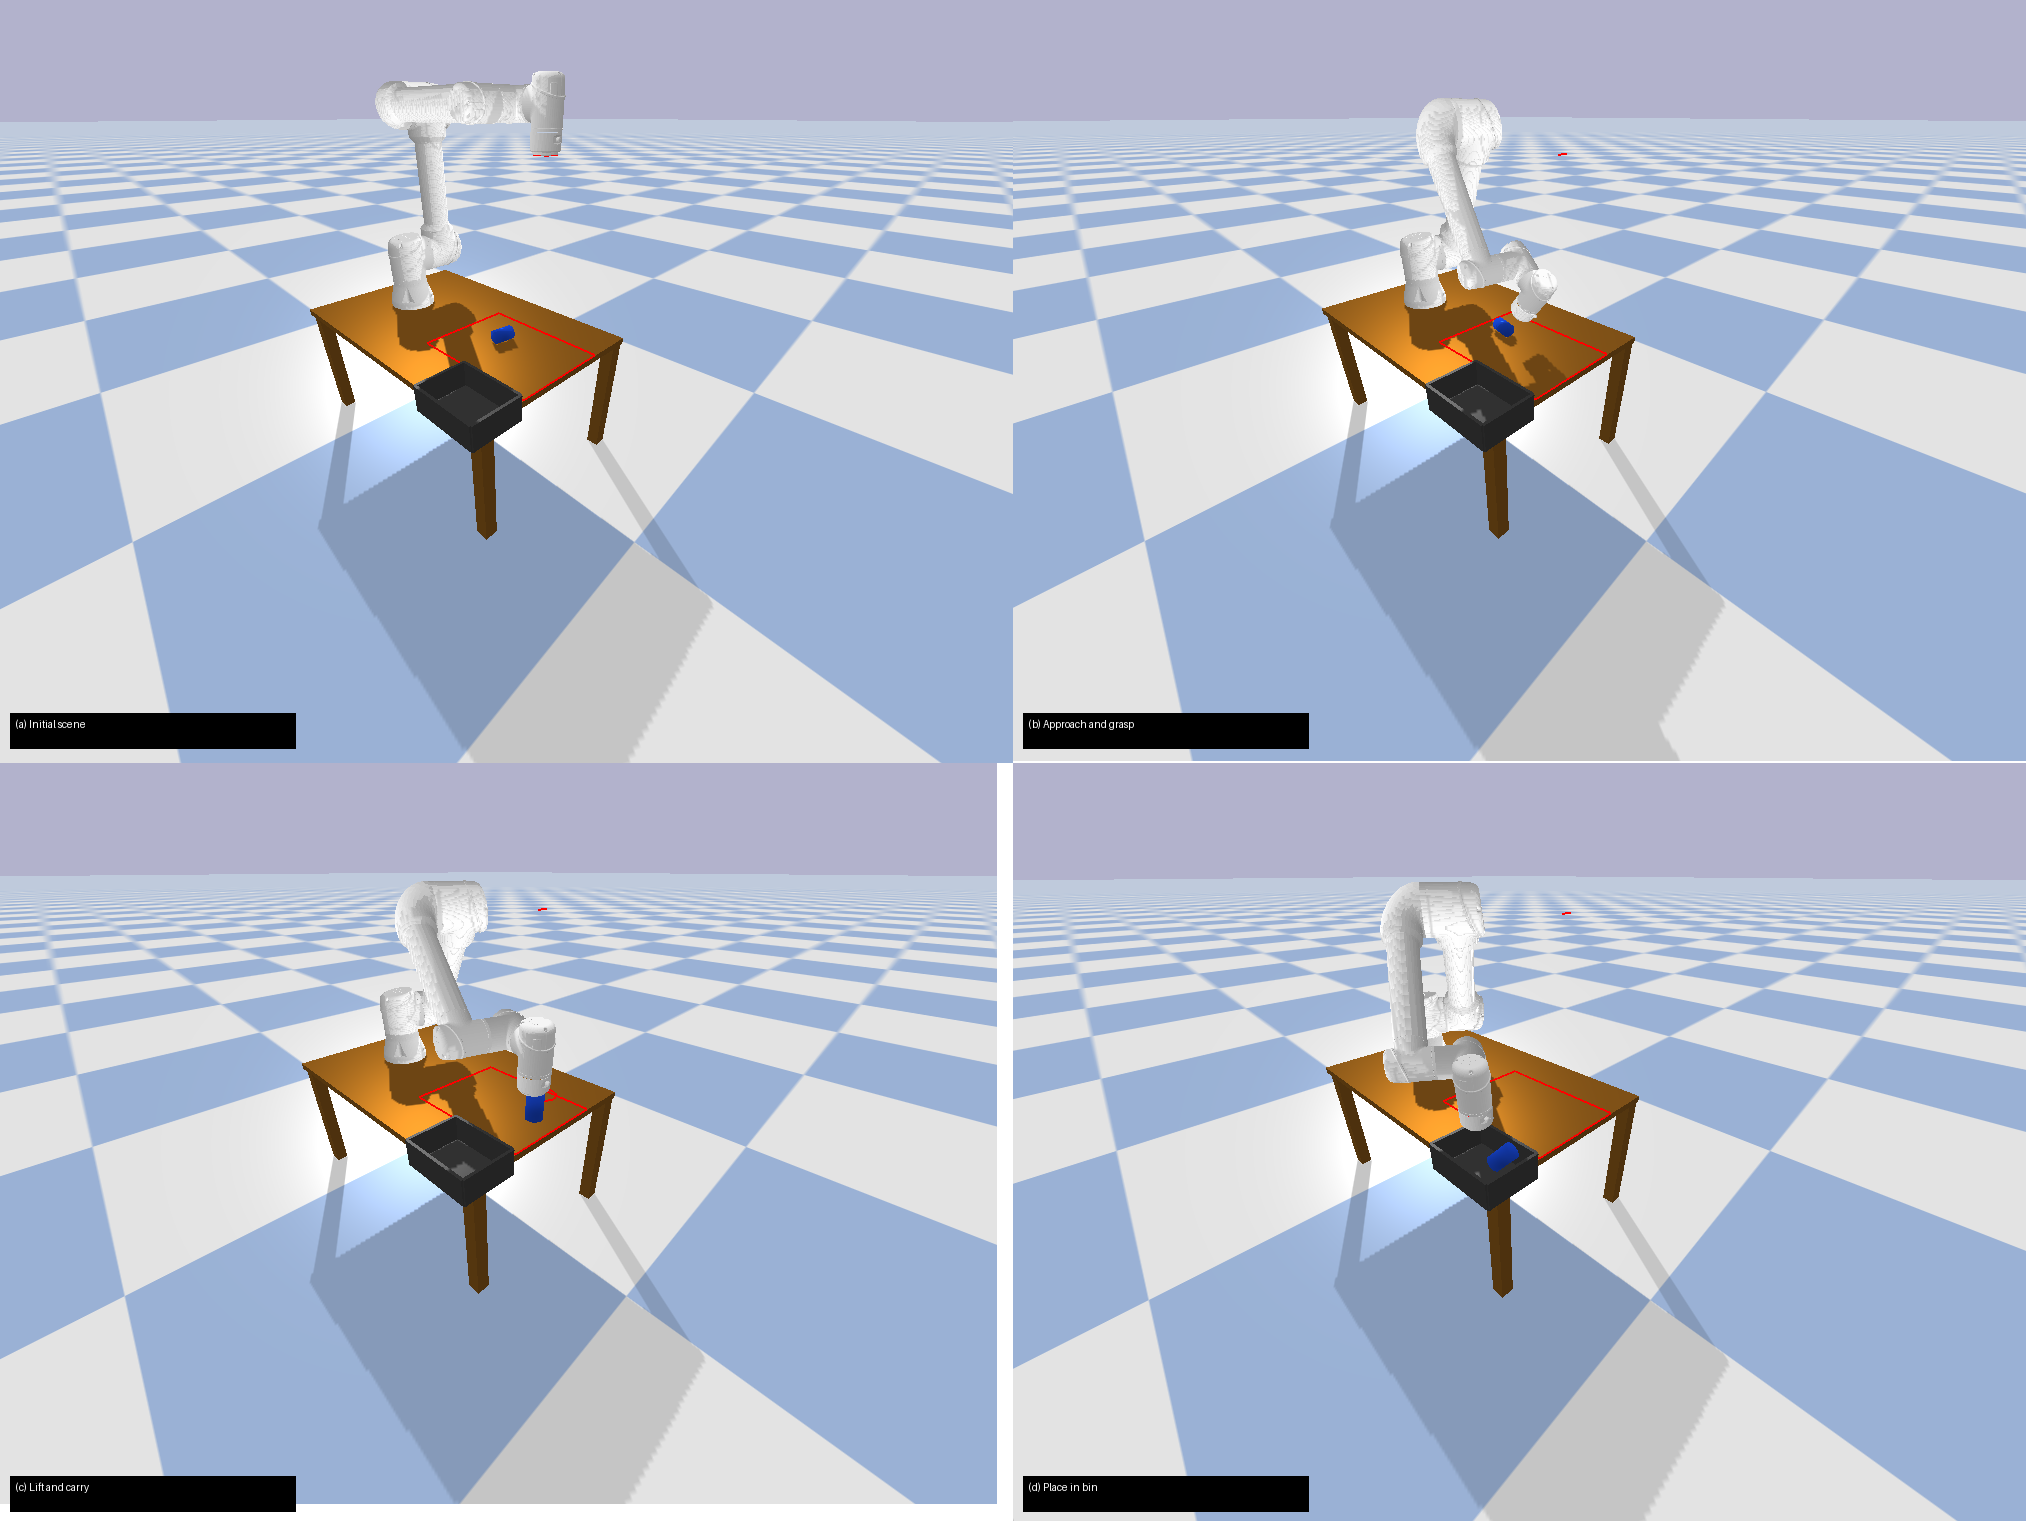
\includegraphics[width=0.90\textwidth]{figures/demo_sequence.png}
\caption{Chuỗi các pha hành động của robot UR5e thực hiện gắp thả vật thể nằm ngang trong PyBullet bao gồm: (a) Cảnh khởi tạo, (b) Tiếp cận và gắp vật, (c) Nâng và vận chuyển vật qua không trung, (d) Thả vật chính xác vào thùng chứa mục tiêu.}
\label{fig:demo_sequence}
\end{figure*}

\begin{itemize}
    \item \textit{Pha (a) Cảnh khởi tạo (Initial scene)}: Vật thể hình trụ được sinh ra ở tư thế nằm ngang ngẫu nhiên trên mặt bàn. Đầu gắp của robot UR5e xuất phát từ vị trí nghỉ Home Pose ở phía trên cao.
    \item \textit{Pha (b) Tiếp cận và gắp vật (Approach and grasp)}: Nhờ các ràng buộc hướng và phần thưởng dẫn đường Pha 0, đầu gắp tự động hướng thẳng đứng xuống dưới bàn, di chuyển nhanh đến sát vị trí vật thể và tự động tạo liên kết gắp chặt vật thể khi khoảng cách đạt dưới 4.5 cm mà không gây va chạm mạnh làm dịch chuyển vật.
    \item \textit{Pha (c) Nâng và vận chuyển (Lift and carry)}: Sau khi gắp được vật, tác tử nhận điểm thưởng gắp và nhanh chóng nâng vật thể lên cao quá 0.20 m để nhận điểm thưởng nâng. Sau đó, tác tử duy trì cao độ đầu gắp trên mức 0.60 m để tránh hình phạt cao độ thấp và nhanh chóng điều hướng vật thể đi qua không gian phía trên mặt bàn hướng về phía thùng chứa.
    \item \textit{Pha (d) Thả vật vào thùng (Place in bin)}: Khi tiến sát vào vùng không gian của thùng chứa, tác tử hạ thấp độ cao đầu gắp để đưa vật vào lòng thùng. Khi đầu gắp tiến sát tâm thùng dưới 5 cm, hệ thống tự động nhả liên kết để vật thể rơi an toàn vào đáy thùng chứa, hoàn thành chu kỳ làm việc.
\end{itemize}

\subsection{Thảo luận về vai trò của các thành phần thiết kế đề xuất}
Các thành phần thiết kế sau được đưa vào với mục tiêu hỗ trợ quá trình học và được xem là các giả thuyết cần được kiểm chứng thêm bằng thí nghiệm khử thành phần:
\begin{itemize}
    \item \textit{Tay gắp lai}: Giúp giảm bớt việc học các hành động đóng mở rời rạc, làm giảm sự phức tạp của không gian tìm kiếm hành động và hạn chế hành vi đóng mở liên tục không mong muốn của tay gắp để nhận thưởng.
    \item \textit{Ràng buộc hướng}: Ràng buộc góc cổ tay $\pm15^\circ$ giúp định hướng giác hút tiếp cận vật theo tư thế phù hợp, đồng thời giới hạn các tư thế đích gửi đến bộ giải IK của PyBullet trong vùng vận hành an toàn.
    \item \textit{Phân chia pha phần thưởng}: Hạn chế vấn đề thưa thớt phần thưởng của chuỗi thao tác dài mà không làm mất đi tính định hướng tổng thể của tác vụ nhờ vào việc chuyển pha dựa trên trạng thái vật lý thực của robot.
\end{itemize}

\subsection{Giới hạn nghiên cứu hiện tại}
Mặc dù hệ thống không ghi nhận episode thất bại trong môi trường thử nghiệm với cấu hình huấn luyện, chúng tôi cần thảo luận các giới hạn biên của kết quả này:
\begin{itemize}
    \item \textit{Phạm vi đánh giá}: Khả năng hoạt động tốt chỉ được ghi nhận trên cấu hình phân phối vật thể mức khó trung bình (\texttt{difficulty=1}) với phân phối vật thể trùng với phân phối huấn luyện. Hệ thống chưa được kiểm chứng hiệu suất trên cấu hình khó hơn (\texttt{difficulty=2}), vật thể có kích thước hoặc khối lượng khác biệt, thùng chứa đổi vị trí, hoặc môi trường có chướng ngại vật di động.
    \item \textit{Tính đại diện thống kê}: Toàn bộ kết quả được báo cáo từ một seed huấn luyện duy nhất (seed 42). Để khẳng định tính ổn định của phương pháp, cần lặp lại thí nghiệm trên nhiều seed độc lập.
    \item \textit{Thiếu nghiên cứu khử thành phần (ablation study)}: Mặc dù bài báo đề xuất tay gắp lai, ràng buộc hướng và phân chia pha phần thưởng là các đóng góp chính, chúng tôi chưa thực hiện so sánh có kiểm soát để đo lường đóng góp riêng lẻ của từng thành phần. Các thí nghiệm khử thành phần và so sánh với baseline (phần thưởng thưa, không ràng buộc hướng, không tay gắp lai) sẽ giúp làm rõ mức độ ảnh hưởng của mỗi thiết kế.
    \item \textit{Chiều hành động dư thừa}: Vector hành động khai báo 7 chiều nhưng chiều thứ 7 ($a_{gripper}$) không tác động lên môi trường do cơ chế tay gắp lai thay thế. Chiều hành động thứ bảy không tạo ra tác động nhân quả lên trạng thái kế tiếp hoặc phần thưởng của môi trường. Do đó, về lý tưởng giá trị Q không phụ thuộc vào chiều này; tuy nhiên, việc duy trì nó vẫn làm tăng số chiều phân phối chính sách và có thể làm giảm hiệu quả khám phá, ảnh hưởng nhẹ đến hiệu quả học.
    \item \textit{Quan sát không đầy đủ}: Vector quan sát 20 chiều không bao gồm vận tốc khớp, vận tốc vật thể hay trạng thái pha rõ ràng. Về mặt lý thuyết, hệ thống gần với mô hình POMDP hơn là MDP quan sát đầy đủ. Việc bổ sung các thông tin động học này có thể cải thiện thêm hiệu suất học.
    \item \textit{Thông tin trạng thái từ mô phỏng}: Tác tử nhận thông tin tọa độ vị trí và hướng của vật thể trực tiếp từ lõi mô phỏng PyBullet. Trong hệ thống thực tế, thông tin này phải được ước lượng thông qua cảm biến camera chiều sâu, điều này sẽ đưa thêm sai số vào hệ thống.
    \item \textit{Chưa kiểm chứng trên robot thật}: Nghiên cứu này chưa triển khai trên cánh tay robot UR5e vật lý và chưa thực hiện các kỹ thuật thu hẹp khoảng cách mô phỏng thực tế (sim to real gap) như Domain Randomization \cite{tobin2017domain}.
\end{itemize}

\section{Kết luận và Hướng phát triển}
Nghiên cứu này đã trình bày chi tiết phương pháp thiết kế và xây dựng môi trường học tăng cường sử dụng thuật toán SAC cho robot UR5e thực hiện tác vụ điều hướng quỹ đạo Cartesian phục vụ gắp thả vật thể trong mô phỏng PyBullet. Bài toán được mô hình hóa xấp xỉ theo quy trình quyết định Markov với quan sát 20 chiều và vector hành động 7 chiều (trong đó 6 chiều Cartesian vi phân thực sự điều khiển robot và chiều thứ bảy dư thừa không sử dụng). Bằng việc đề xuất cơ chế tay gắp lai tự động hóa logic hút thả dựa trên điều kiện hình học, bộ ràng buộc hướng đầu gắp chống xoắn khớp và hàm phần thưởng định hướng phân chia theo 3 pha hoạt động cụ thể, chính sách điều hướng của tác tử đã hội tụ sau 600,000 bước huấn luyện từ đầu trên một seed duy nhất. Đánh giá thực nghiệm trên cấu hình \texttt{difficulty=1} ghi nhận không có episode thất bại với chu kỳ thực thi trung bình dưới 29 bước thời gian.

Trong thời gian tới, hướng nghiên cứu chính sẽ tập trung vào việc thu hẹp khoảng cách từ mô phỏng vào thực tế. Chúng tôi dự kiến tích hợp các thuật toán xử lý ảnh từ camera chiều sâu để ước lượng tư thế vật thể thay vì lấy thông tin trực tiếp từ simulator. Đồng thời, chúng tôi sẽ áp dụng kỹ thuật Domain Randomization để ngẫu nhiên hóa các tham số vật lý của mô phỏng như khối lượng, ma sát, độ trễ truyền động và sai số cảm biến nhằm chuẩn bị cho việc chuyển giao chính sách điều khiển lên cánh tay robot UR5e vật lý trong phòng thí nghiệm.

\begingroup
\sloppy
\bibliographystyle{IEEEtran}
\bibliography{references}
\endgroup

\end{document}
